\section{Gapped Phases with Symmetries}

Our discussion thus far has been general, but often we are interested in systems with certain symmetries $\set{S^g: g \in G}$ where $s^g$ are unitary or anti-unitary operators (though the only example we will discuss in any depth will be unitary). We are interested in classes of Hamiltonians $\set{H}$ that satisfy $[H, S^g] = 0$. Thus, we really only want to consider the subclass of Hamiltonians in our phase diagram which have this symmetry; this changes the phase diagram as it is no longer sufficient to have a gapped path between two Hamiltonians, but a gapped path that preserves the symmetry, as well.

\subsection{Defining Gapped Phases with Symmetry}

\textit{Definition (gapped phases with symmetries).} Two symmetric local gapped Hamiltonians $H_a, H_b$ belong to the same phase if they can be connected by a \emph{symmetric} local gapped path $\set{H(s): 0 \leq s \leq 1}$.

\begin{center}
    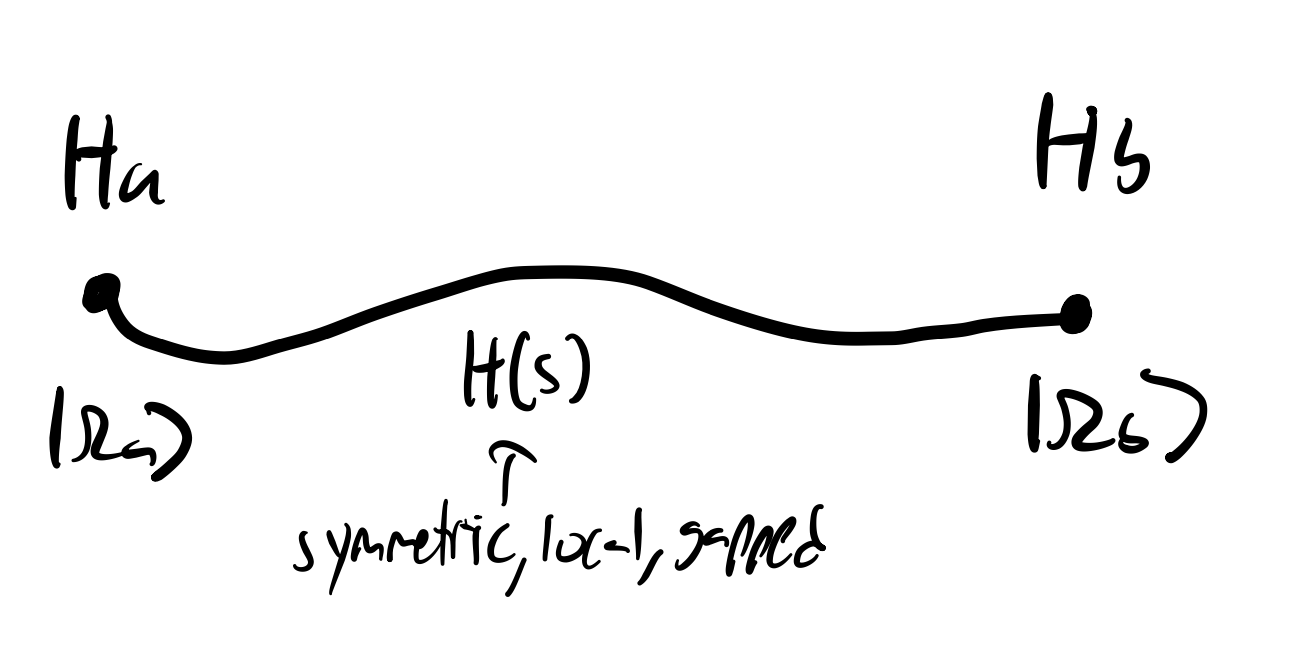
\includegraphics[scale=0.35]{Lectures/Images/lec13-sympath.png}
\end{center}

The motivation for the path being symmetric is that all qualitative properties related to the symmetries should be shared by the two connected Hamiltonians. Note that this is a more restrictive definition of a phase. You may have a gapped path between the Hamiltonians that breaks the symmetries, but not that preserves one. Then, the properties of the Hamiltonians that do not have to do with the symmetries will be shared.

We can give an equivalent state-centric definition, as we did for gapped phases last lecture:

\textit{Definition (gapped phases with symmetries).} $H_a, H_b$ belong to the same phase if and only if their ground states $\ket{\Omega_a}, \ket{\Omega_b}$ are connected by a symmetric local unitary:
\begin{equation}
    \ket{\Omega_b} = U\ket{\Omega_a}
\end{equation}
\begin{equation}
    U = \mathcal{T}\exp(-i\int_0^T H(t)dt)
\end{equation}
with $[H(t), S^g] = 0$ for all $t$. Note that this implies that $[U, S^g] = 0$, but requiring $[H(t), S^g] = 0$ is a stronger condition than just requiring $[U, S^g] = 0$.

Generally, symmetry enriches phase diagrams, because we can have more subtle distinctions between systems that relate to some symmetry.

\subsection{Symmetry-protected topological phases}
This is the simplest class of gapped phases with symmetry (other than perhaps symmetry-broken phases).

\textit{Definition (SPT phases).} A local gapped Hamiltonian $H$ with symmetries $\set{S^g: g \in G}$ belongs to a non-trivial SPT phase if $H$ has a unique ground state $\ket{\Omega}$ (on an infinite, or periodic lattice, i.e. without boundaries), and:
\begin{enumerate}
    \item There exists a local gapped path connecting $H$ with a ``trivial'' Hamiltonian, i.e. a Hamiltonian whose ground state is a product state\footnote{In the case of fermions, one would replace this with an atomic insulator - a state with a fixed number of fermions at each lattice site.} $\ket{\Omega_0}$.
    \begin{center}
        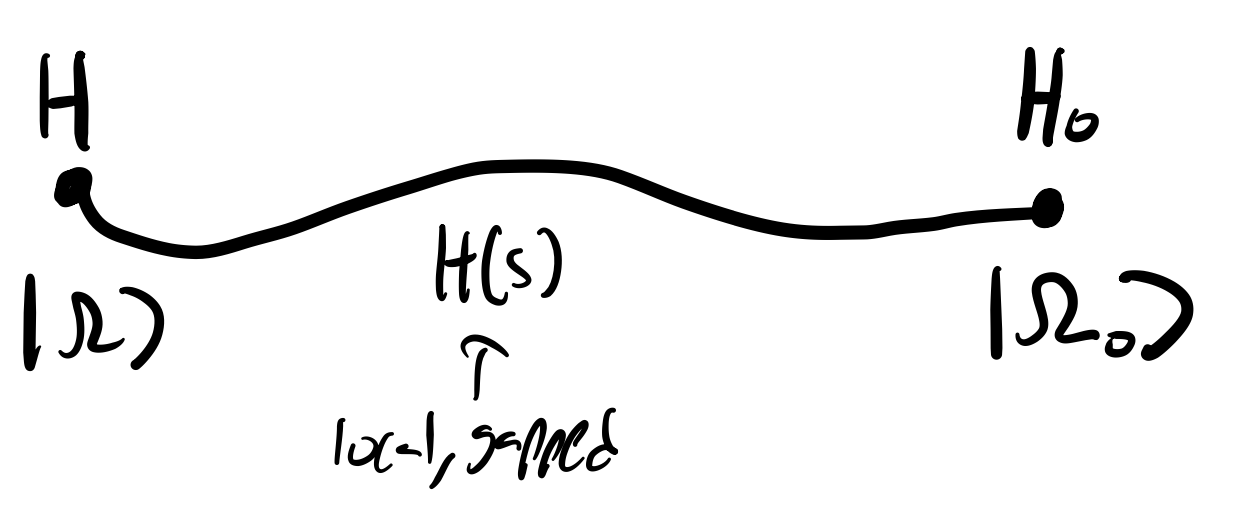
\includegraphics[scale=0.35]{Lectures/Images/lec13-path.png}
    \end{center}
    \item There does \emph{not} exist a local, gapped, symmetric path connecting $H$ with the trivial Hamiltonian $H_0$.
    \begin{center}
        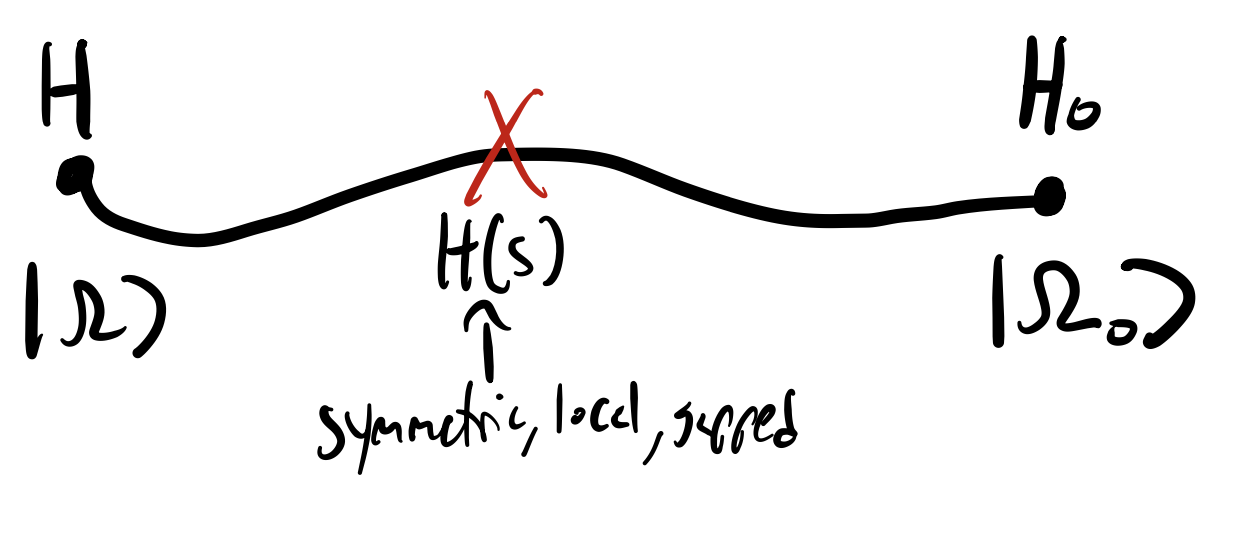
\includegraphics[scale=0.35]{Lectures/Images/lec13-nosympath.png}
    \end{center}
\end{enumerate}
In other words, the symmetry protects/prevents you from smoothly deforming the Hamiltonian to a trivial one.

Again, there is an analogous definition in terms of local unitaries acting on states:

\textit{Definition (SPT phases).} $H$ belongs to a non-trivial SPT phase if its unique ground state $\ket{\Omega}$ satisfies:
\begin{enumerate}
    \item $\ket{\Omega}$ can be connected to a product state by a local unitary $U$, i.e. $\ket{\Omega} = U\ket{\Omega_0}$. Recall that we called such states \emph{short-range entangled}, so this condition on the definition tells us that all states with SPT order are short-range entangled.
    \item $\ket{\Omega}$ cannot be connected to a product state by a \emph{symmetric} local unitary $U$, i.e. $\ket{\Omega} \neq U\ket{\Omega_0}$ for $U$ symmetric and local ($[H(t), S^g] = 0$ for all $t$).
\end{enumerate}

One other comment; here we defined a \emph{non-trivial} SPT phase. Trivial SPT phases are those that obey 1 but not 2, in other words we can find a symmetric path that connects the Hamiltonian to a product state Hamiltonian, or a symmetric local unitary that connects the ground state to a product state.

This is an abstract definition, but there are many examples of SPT - for example topological insulators, which were in part responsible for the renaissance. But our first/simplest example will be that of the 1-D cluster state\footnote{The other classic example is the AKLT chain, but the cluster state has the benefit of being exactly solvable}.

\subsection{1-D cluster state}
We consider a chain of qubits, with Hamiltonian:
\begin{equation}
    H_c = -\sum_i Z_{i-1}X_iZ_{i+1}
\end{equation}
\begin{center}
    
\includegraphics[scale=0.35]{Lectures/Images/lec13-clusterchain.png}
\end{center}
The system has two symmetries $S_e, S_o$:
\begin{equation}
    \begin{split}
        S_e &= \prod_{i}X_{2i}
        \\ S_o &= \prod_{i}X_{2i+1}
    \end{split}
\end{equation}
These symmetries are Ising-like as they correspond to spinflips on even/odd sublattices. $S_e, S_o$ square to 1 and commute, thus we can say that $H$ has a $\ZZ_2 \times \ZZ_2$ symmetry, with the $S_e, S_o$ being the generators. We will see that $H$ belongs to a nontrivial SPT phase with this symmetry.

First, let us solve the model. Notice that:
\begin{equation}
    [Z_{i-1}X_iZ_{i+1}, Z_{j-1}X_jZ_{j+1}] = 0
\end{equation}
If the terms do not overlap, they obviously commute. If they overlap across one spin, the two $Z$s also clearly commute. If they overlap across two spins, we have two anticommuting pairs of $X, Z$ so overall the operators indeed commute.

Since all terms in the Hamiltonian commute, they can be simultaneously diagonalized (and they have eigenvalues $\pm 1$ since each term squares to identity), so the ground states obey:
\begin{equation}
    (Z_{i-1}X_iZ_{i+1})\ket{\Omega} = \ket{\Omega}
\end{equation}
We are faced with the same question we faced in the toric code; we have the condition for the ground states, but how many ground states are there? It ultimately depends on the geometry. But in the case of the infinite lattice or the periodic chain, we can check that there is a unique state. The periodic case can be checked via the trace calculation. The infinite chain, we can explicitly construct the ground state. We've seen them before, so we won't do it here. In a few minutes we will do an alternative calculation that implies the uniqueness of the ground state. But, taking this to be true, we have a unique ground state $\ket{\Omega}$ and a gap of $\Delta = 2$ (corresponding to the flip of a single stabilizer).

Thus far, we have verified that the Hamiltonian has a unique ground state and a gap. But, to show that the cluster state Hamiltonian belongs to a nontrivial SPT phase, we need to show that (1) $\ket{\Omega}$ is short-range entangled and (2) That there exists no symmetric local unitary that connects it to the product state.

\subsection{1-D cluster state is SRE}
Define a 2-qubit unitary:
\begin{equation}
    CZ_{1,2} = \frac{\II + Z_1 + Z_2 - Z_1Z_2}{2}
\end{equation}
or equivalently:
\begin{equation}
    \begin{split}
        CZ\ket{\uparrow\uparrow} &= \ket{\uparrow\uparrow}
        \\ CZ\ket{\uparrow\downarrow} &= \ket{\uparrow\downarrow}
        \\ CZ\ket{\downarrow\uparrow} &= \ket{\downarrow\uparrow}
        \\ CZ\ket{\downarrow\downarrow} &= -\ket{\downarrow\downarrow}
    \end{split}
\end{equation}
which makes it clear why this is called a ``controlled-$Z$'' gate. We can check that $(CZ)^2 = 1$ (obvious from the definition), and also that:
\begin{equation}
    \begin{split}
        (CZ)Z_1(CZ) = Z_1
        \\ (CZ)Z_2(CZ) = Z_2
        \\ (CZ)X_1(CZ) = X_1Z_2
        \\ (CZ)X_2(CZ) = Z_1X_2
    \end{split}
\end{equation}
Now, define:
\begin{equation}
    U = \prod_i(CZ)_{i, i+1}
\end{equation}
which is a depth-2 quantum circuit:

\begin{center}
    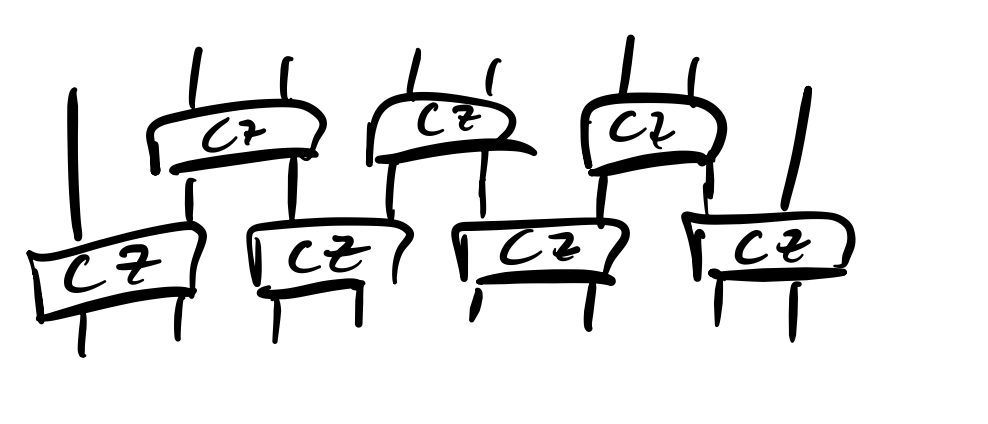
\includegraphics[scale=0.35]{Lectures/Images/lec13-czcircuit.png}
\end{center}

which is special case of a local unitary. In this case the action is equivalent to a translation-invariant two-body Ising interaction for a fixed time.

The claim is that:
\begin{equation}
    \ket{\Omega} = U\ket{\set{X_i = 1}}
\end{equation}
which shows that $\ket{\Omega}$ is SRE since $\ket{\set{X_i = 1}}$ is a product state and $U$ is finite-depth quantum circuit.

To prove the claim, note that:
\begin{equation}
    (CZ)_{i-1, i}(CZ)_{i, i+1}X_i(CZ)_{i, i+1}(CZ)_{i-1, i} = (CZ)_{i-1, i}X_i Z_{i+1}(CZ)_{i-1, i} = (CZ)_{i-1, i}X_i (CZ)_{i-1, i}Z_{i+1} = Z_{i-1}X_iZ_{i+1}
\end{equation}

Thus:
\begin{equation}
    UX_i U^\dag = Z_{i-1}X_iZ_{i+1}
\end{equation}
which implies that the ground state of $H_0 = -\sum_i X_i$ gets mapped to the ground state of $H_c = -\sum_i Z_{i-1}X_iZ_{i+1}$. More explicitly:
\begin{equation}
    UX_iU^\dagger \ket{\Omega} \implies X_i U^\dagger \ket{\Omega} = U^\dag \ket{\Omega} \implies U^\dag \ket{\Omega} = \ket{\set{X_i = 1}}
\end{equation}
and thus:
\begin{equation}
    \ket{\Omega} = U\ket{\set{X_i = 1}}.
\end{equation}
so $U$ has the desired property of mapping from the product state to the cluster state. Also note in particular that since $H_0 = -\sum_i X_i$ has a unique ground state and a gap, this immediately implies that so does $H_c$.

Note that the $CZ$ gates are \emph{not} $\mathbb{Z}_2 \times \mathbb{Z}_2$ symmetric. Recalling:
\begin{equation}
    (CZ)_{i, i+1} = \frac{\II + Z_i + Z_{i+1} - Z_iZ_{i+1}}{2}
\end{equation}
we can see that $[(CZ)_{i, i+1}, S_{e/o}] \neq 0$ (as the symmetries flip some of the signs). This is crucial. If the gates were $\mathbb{Z}_2 \times \mathbb{Z}_2$-symmetric, then each gate could be generated by a symmetric 2-qubit Hamiltonian, and hence $U$ would be a symmetric local unitary, implying that the cluster state was in the trivial SPT phase.

This isn't enough to show that the cluster state is in a non-trivial SPT, as in order to do this we need to show that no local symmetric unitary exists such that $\ket{\Omega} = U\ket{\Omega_0}$ for $\ket{\Omega_0}$ a product state. This will be left as an exercise on your homework. But after this, we will be able to conclude that $H_c$ and its ground state $\ket{\Omega}$ are in a non-trivial SPT phase.

As an aside - it actually turns out that the unitary $U$ does satisfy $[U, S_{e/o}] = 0$. This does \emph{not} imply that $U$ is a symmetric local unitary.

Next lecture, we will explore the physical properties of the cluster state that makes it nontrivial - we will see this when we add boundaries, as we will see that we get a robust, 4-fold degeneracy - 0 energy excitations at the boundary.